%
% fast.tex
%
% (c) 2019 Prof Dr Andreas Müller, Hochschule Rapperswil
%
\section{Der schnelle Waveletalgorithmus
\label{section:fast}}
\rhead{Der schnelle Waveletalgorithmus}
Die spezielle Struktur der Multiskalenanalyse ermöglicht, die Analyse
bezüglich einer Waveletbasis besonders effizient durchzuführen.
Es zeigt sich, dass der Rechenaufwand für die Transformation linear
mit der Anzahl der Samples wächst.
Dies ist deutlich schneller als zum Beispiel bei der Fourier-Transformation.

\subsection{Approximation und Detail}
Wir betrachten zunächst einen einzelnen Vektorraum $V_{j+1}$.
Mit den Basisfunktionen $\varphi_{j,k}$ kann eine Approximation
eines Signals gefunden in $V_{j+1}$ gefunden wurden.
Sie gibt Details der Grössenordnung $2^{-j}$ wieder.
Man erhält die Approximation von $f$ in $V_{j+1}$ aus den sogenannten
{\em Approximationskoeffizienten}
\index{Approximationskoeffizient}%
\[
a_{j,k} = \langle f,\varphi_{j,k}\rangle
\qquad\text{durch}\qquad
f\simeq \sum_{k} a_{j,k} \varphi_{j,k}.
\]
Im Vektorraum $V_{j+1}$ ist aber noch mehr Information über eine Funktion
verfügbar.
Die Basisfunktion $\psi_{j,k}$ geben die Details eines Signals nahe bei
$t=k2^{-j}$ mit einer Auflösung von der Grössenordnung $2^{-j-1}$ wieder.
Je grösser $j$, desto feiner die Auflösung.
Die sogenannten {\em Detailkoeffizienten}
\index{Detailkoeffizient}%
\[
b_{j,k} = \langle f,\psi_{j,k}\rangle
\]
repräsentieren die Detailinformation.

Aus Approximations- und Detailkoffizienten lässt sich ein Signal in
$f\in V_{j+1}$ mit 
\[
f
=
\sum_{k} a_{j,k}\varphi_{j,k} + \sum_k b_{j,k}\psi_{j,k}
=
\sum_{k} \langle f,\varphi_{j,k}\rangle\cdot \varphi_{j,k}
+
\sum_k \langle f,\psi_{j,k}\rangle\cdot \psi_{j,k}
\]
vollständig rekonstruieren.
Die Analyse des Signals erfordert also im Prinzip die Berechnung eines
Skalarproduktes für jeden Koeffizienten $a_{j,k}$ und $b_{j,k}$.
In dieser Form scheint die Waveletanalyse kaum praktisch durchführbar.

\subsection{Sampling}
In der Praxis liegen die Daten nicht in kontinuierlicher Form vor, sondern
nur als eine Folge von Samples.
Die Auflösung dieser Samples ist die höchste erreichbare Approxmationsstufe.
Sie sollten daher alleine durch $a$-Koeffizienten dargestellt werden können.
Sei $N$ derart, dass die Samples die Zeitauflösung $2^{-N}$ haben (dies
entspricht der Wahl einer Masseinheit für das Sampling-Intervall).
Wie hängen die $a_{N,k}$ mit den Samplewerten zusammen?

Für grosses $j$ ist die Funktion $\varphi_{j,k}$ in der Nähe von $2^{-j}k$
konzentriert.
Ändert das Signal $f$ in einer Umgebung von $2^{-j}k$ nur wenig, kann man
\begin{equation*}
a_{j,k}
=
\langle f,\varphi_{j,k}\rangle
=
\int_{-\infty}^\infty f(t)\, \varphi_{j,k}(t)\,dt
\simeq
f(2^{-j}k)
\int_{-\infty}^\infty \varphi_{j,k}(t)\,dt
\end{equation*}
approximieren.
Bis auf einen möglichen skalaren Faktor gegeben durch das Integral, sind
die Koeffizienten $a_{j,k}$ für genügend grosses $j$ also durch
Sample-Werte $f(2^{-j}k)$ ausreichend genau approximiert.
Es ist daher zulässig, die $a_{N,k}$ als die Samplewerte des Signals
zu betrachten.

\subsection{Berechnung der Koeffizienten als Filter}
Ein praktisch nützlicher Analyse-Algorithmus muss jetzt die Koeffizienten
\[
\begin{aligned}
a_{j,k}
&=
\langle f, \varphi_{j,k}\rangle
=
\langle f, D_{2^{-j}}T_k\varphi \rangle
&&&&\text{Approximation}
\\
b_{j,k}
&=
\langle f, \psi_{j,k}\rangle
=
\langle f, D_{2^{-j}}T_k\psi \rangle
&&&&\text{Detail}
\end{aligned}
\]
für jedes beliebige Signal $f$ auf effiziente Art berechnen können.
Als Basis für die Berechnung stehen die Samplewerte $a_{N,k}$ zur 
Verfügung.
In der Berechnung kann verwendet werden, dass die Funktionen
$\varphi_{j,k}$ eine orthonormierte Basis von $V_j$ sind
und die $\psi_{j,k}$ eine orthonormierte Basis von $W_j$.

\begin{figure}
\centering
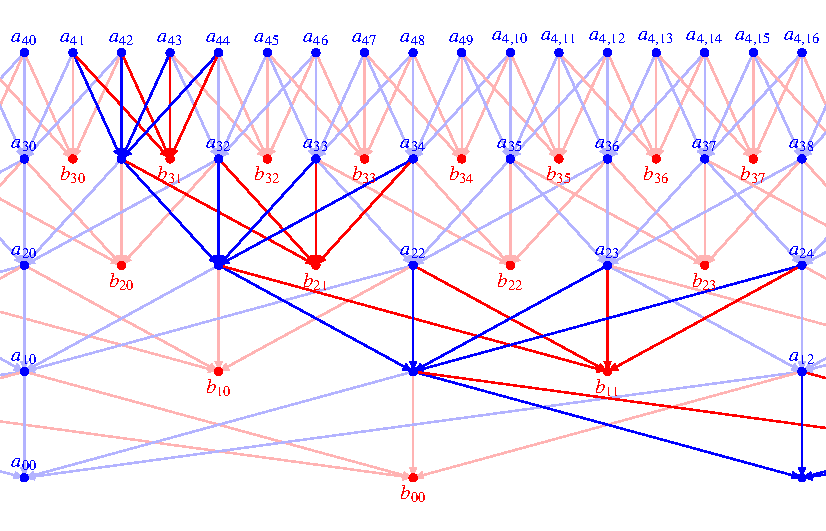
\includegraphics{chapters/7-algo/images/fastalgo.pdf}
\caption{Datenfluss für die Analyse mit vier von $0$ verschiedenen
Koeffizienten $\color{blue}\bar{h}_{-1},\dots,\bar{h}_2$ und
$\color{red}\bar{g}_{-1},\dots,\bar{g}_2$.
Ausgangsdaten für die Analyse sind die Samples $\color{blue}a_{4k}$
in der ersten Zeile.
Durch Anwendung der $\color{blue}h$-Koeffizienten (blaue Linien) können daraus
die Mittelwerte mit gröberer Auflösung $\color{blue}a_{3k}$ gewonnen werden.
Ebenso können durch Anwendung der $\color{red}g$-Koeffizienten (rote Linien)
die Detail-Koeffizienten $\color{red}b_{3k}$ gefunden werden.
Dies wird für jede weitere Detail-Ebene $j$ wiederholt: aus den Koeffizienten
$\color{blue}a_{jk}$ werden mit den $\color{blue}h$-Koeffizienten die
$\color{blue}a_{j+1,k}$ und mit den $\color{red}g$-Koeffizienten die
$\color{red}b_{j+1,k}$ bestimmt.
\label{algo:image:fastalgo}}
\end{figure}

Das Schlüsselelement einer Multiskalen-Analyse ist die Skalierungsrelation
\begin{align}
\varphi(t) &= \sqrt{2} \sum_{l\in\mathbb Z} h_l \varphi(2t-l)
\notag
\intertext{oder mit den Operatoren $D$ und $T$ geschrieben:}
\varphi    &= \sum_{l\in\mathbb Z} h_l D_{\frac12}T_l\varphi.
\label{algo:formel:phiscale}
\end{align}
Da die Skalierung $D_{\frac12}$ jeden der Vektorräume $V_j$ isometrisch
auf $V_{j+1}$ abbildet, wird daraus eine Skalierungsrelation für alle
Basisfunktionen $\varphi_{j,k}$, die durch Anwendung des Operators
$D_{2^{-j}}T_k$ auf \eqref{algo:formel:phiscale} gefunden werden kann:
\begin{equation}
\varphi_{j,k}
=
D_{2^{-j}}T_k\varphi
=
\sum_{l\in\mathbb Z} h_l D_{2^{-j}} T_k D_{\frac12}T_l \varphi
=
\sum_{l\in\mathbb Z} h_l D_{2^{-j}} D_{\frac12}T_{2k}T_l \varphi
=
\sum_{l\in\mathbb Z} h_l D_{2^{-j-1}} T_{l+2k} \varphi
=
\sum_{l\in\mathbb Z} h_l \varphi_{j+1,l+2k}.
\label{fast:phirelation}
\end{equation}
Im zweitletzten Schritt haben wir die Vertauschungsrelation
$D_{\frac12}T_{2k}=T_{\frac12\cdot2k}D_{\frac12}=T_kD_{\frac12}$
für 
$D_{\frac12}$ und $T_k$ verwendet.
Ausserdem folgt aus der Tatsache, dass $W_j\subset V_{j+1}$ ist,
dass die Basisfunktionen $\psi_{j,k}$ der Orthonormalbasis von $W_j$
Linearkombinationen der Funktionen $\varphi_{j+1,l}$ sein müssen,
die wir als Relation
\[
\psi(t) = \sqrt{2}\sum_{l\in\mathbb Z} g_l \varphi(2t-l),
\]
für das Mutterwavelet schreiben.
Wieder mit Hilfe der Skalierungsisometrien $D_{2^{-j}}$ und den
Translationen $T_k$  folgt die entsprechende Relation
\begin{equation}
\psi_{j,k}
=
\sum_{l\in\mathbb Z} g_l D_{2^{-j-1}}T_{l+2k}\varphi
=
\sum_{l\in\mathbb Z} g_l \varphi_{j+1,l+2k}
\label{fast:psirelation}
\end{equation}
für die skalierten und verschobenen Wavelets.

Wendet man die Relationen \eqref{fast:phirelation} und \eqref{fast:psirelation}
auf die Analyse des Signals $f$ an, indem man das Skalarprodukt mit $f$ bildet,
findet man die Beziehungen
\begin{align}
a_{j,k}
=
\langle f,\varphi_{j,k} \rangle
&=
\sum_{l\in\mathbb Z} \bar{h}_l \langle f,\varphi_{j+1,l+2k}\rangle
=
\sum_{l\in\mathbb Z} \bar{h}_l a_{j+1,l+2k}
\label{fast:akoefgleichung}
\\
b_{j,k}
=
\langle f,\psi_{j,k} \rangle
&=
\sum_{l\in\mathbb Z} \bar{g}_l \langle f,\varphi_{j+1,l+2k}\rangle
=
\sum_{l\in\mathbb Z} \bar{g}_l a_{j+1,l+2k}
\label{fast:bkoefgleichung}
\end{align}
für die Koeffizienten $b_{j,k}$ und $a_{j,k}$.
Die Formeln drücken die Wavelet-Koeffizienten für die Auflösung $j$ durch
die Wavelet-Koeffizienten für die Auflösung $j+1$ aus.
Sobald die Koeffizienten $a_{N,k}$ bekannt sind, können zunächst
alle Koeffizienten $a_{N-1,k}$ und weiter alle
$a_{j,k}$ mit $j<N$ berechnet werden.

Die Gleichungen \eqref{fast:akoefgleichung} und \eqref{fast:bkoefgleichung}
beschreiben den in Abbildung~\ref{algo:image:fastalgo} illustrierten
Algorithmus, der aus den Samples $a_{N,k}$ schrittweise die
Detail-Information $b_{N-1,k}$, $b_{N-2,k}$ und so weiter extrahiert.
In jedem Schritt ist pro Koeffizient gleich viel neue Arbeit erforderlich,
nämlich je eine Auswertung der Summe \eqref{fast:akoefgleichung}, die die
Approximationskoeffizienten bereitstellt und eine Auswertung der Summe
\eqref{fast:bkoefgleichung}, welche die Detailkoeffizienten extrahiert.
Man kann auch erkennen, dass jede Detailebene insgesamt halb so viel
Arbeit erfordert wie die darüberliegende Ebene.

Die Waveletanalyse, durchgeführt nach \eqref{fast:akoefgleichung}
und \eqref{fast:bkoefgleichung} hat die Struktur zwier Faltungsfilter mit
\index{Faltungsfilter}%
Koeffizienten $h_k$ und $g_k$, die allerdings nur bei jeder
zweiten Sampleposition angewendet werden.
Solche Filter lassen sich sehr effizient zum Beispiel in einem Signalprozessor
realisieren.
Die speziellen Eigenschaften einer Multiskalenanalyse ermöglichen aber 
weitere Verbesserungen, die in Kapitel~\ref{chapter:fpga} angedeutet werden.

\begin{beispiel}
Die Skalierungsrelation des Haar-Wavelets hat die Koeffizienten
$h_0=h_1=1$, $g_0=1$ und $g_1=-1$.
Die Berechnung der Koeffizienten gemäss \eqref{fast:akoefgleichung}
und \eqref{fast:bkoefgleichung} führt auf das folgende Berechnungsschema:
\[
\xymatrix{
\dots
	&a_{j,-2} \ar[d] \ar[dr]
		&a_{j,-1} \ar@[red][d]^{\color{red}\cdot (-1)} \ar[dl]
			&a_{j,0} \ar[d] \ar[dr]
				&a_{j,1} \ar@[red][d]^{\color{red}\cdot (-1)} \ar[dl]
					&a_{j,2} \ar[d] \ar[dr]
						&a_{j,3} \ar@[red][d]^{\color{red}\cdot (-1)} \ar[dl]
							&\dots
\\
\dots
	&a_{j-1,-1} \ar@[red][d]^{\color{red}\cdot(-1)}
		&b_{j-1,-1}
			&a_{j-1,0}\ar[d] \ar[drr]
				&b_{j-1,0}
					&a_{j-1,1} \ar@[red][d]^{\color{red}\cdot (-1)} \ar[dll]
						&b_{j-1,1}
							&\dots
\\
\dots &b_{j-2,-1} 
		&
			&a_{j-2,0} \ar[d] \ar[drrrr]
				&
					&b_{j-2,0}
						&
							&\dots \ar[dllll]
\\
\dots &
		&
			&a_{j-3,0}
				&
					&
						&
							&\dots
}
\]
Wo immer zwei Pfeile zusammenkommen, müssen die Terme, von denen die
Pfeile ausgehen, summiert werden.
Rote Pfeile multiplizieren die Ausgangsterme zusätzlich mit $-1$.
\end{beispiel}

\subsection{Rechenaufwand}
Wir können die Anzahl der benötigten Operation noch etwas genauer abschätzen.
Sei $n$ die Anzahl der nichtverschwindenden Koeffizienten $h_k$ und $g_k$.
Zur Verarbeitung von $2^N$ Samples sind dann $2\cdot 2^{N-1}\cdot n$
Operationen aus je einer Multiplikation mit dem Koeffizienten und
einer Addition notwendig.
Solche Operationen lassen sich in Hardware besonders effizient realisieren,
da dafür sogenannte MAC-units (Multiply-Accumulate) zur Verfügung stehen.
Auf der nächsten Ebene stehen halb so viele Datenpunkte zur Verfügung,
es bleiben also nur noch $2\cdot 2^{N-2}\cdot n$ Operationen.
Die Gesamtzahl der Operationen ist daher
\[
2^Nn + 2^{N-1}n + 2^{N-2}n+\dots
=
2^Nn\biggl(1+\frac12+\frac14+\dots\biggr)
<
2^Nn\cdot 2
=
2^{N+1}n.
\]
Der Aufwand für $l=2^{\log_2 l}$ Samples ist damit $2ln = O(l)$.
Die Wavelettransformation kann in einer Zeit durchgeführt werden, die 
linear ist in der Länge des Inputs.
Dies ist eine deutliche Verbesserung gegenüber zum Beispiel der
Fourier-Transformation, die auch mit dem FFT-Algorithmus die Zeit
$O(l\log l)$ braucht.
In den Kapiteln~\ref{chapter:fpga} und \ref{chapter:lifting} wird gezeigt,
dass dank einer Faktorisierung der Transformation in sogenannte Lifting Steps
nochmals ein Faktor $2$ an Geschwindigkeit gewonnen werden kann.

